%\pagenumbering{arabic}
\section{系统分析与设计}

在本次答辩系统开发以及通常的软件开发中,需求分析工作指的是在项目开发人员修改或创建一个产品时,确定新系统的开发目的、适用范围、类型定义和具体功能时所需要完成的所有工作。需求分析也是软件开发前期过程中的一个非常必要的过程。在该过程中,软件开发者和系统分析员需要确定该产品使用者的实际需要。只有在确定了这些需要之后,才能够分析和找到软件开发中的具体解决方法。

需求分析对于系统或软件项目的成功至关重要。这些项目应该是文件化的、可操作的、可测量的、可测试的、可追溯的,对已确认的业务需求,其详细程度应被定义为足以用于系统设计的程度。

\subsection{系统需求分析}

在中国的大多数高校,根据规定,任何学生的毕业设计题目在同一年都是不一样的。因此,学院将为学生们准备一些题目。每位学生最终都会经过论文评阅、审阅、项目答辩等一系列工作来得到一个最终得分。学院管理如此大量的数据也是一项挑战。这便需要一个方便、易用的线上信息系统来维护。

因此,答辩系统必须具备 4 个基本模块: 论文评审模块、答辩小组划分模块、答辩分数记录模块以及综合数据浏览模块。系统一共分为 4 种基本角色:管理员、答辩组组长、秘书、普通成员。其中后三种角色均属于答辩小组成员,属于学院教师,并由管理员每年任命。

该系统还需要提供完善的信息导入导出功能,管理员能够按照专业班级来筛选并查看学生的选题结果,以及总览所有专业的选题情况和答辩情况。并且,该系统在以后或许会增加学院教学工作辅助等其他功能,或接入现有的校级教务系统,要求网站系统有良好的可扩展性。同时,该应用环境拥有用户数量大、访问时间集中、实时性强的特点,要求服务器拥有良好的并发处理性能。最后,所开发的系统应该做到操作简易,使业务系统操作不会受到用户电脑知识水平限制。

答辩系统也应具有良好的可维护性。由于项目涉及的信息比较广,数据库中的信息需定期修改,系统可利用的空间资源及计算资源也随之下降,为了使系统能高效地运行和更好地服务于用户,学院可以对系统数据进行简单的维护,以及对一些简单的功能进行二次开发。系统的开放性同样重要,该答辩系统能够在开放的硬件体系结构和软件系统中运行,并且能与之前已完成的 GMS 选题系统顺利连接,不会因外部运行环境的不同而需要额外的修改工作。


\subsection{业务流程图及系统用例图}

流程图是一种表示算法、工作流程或过程的图表。该流程图将步骤显示为各种框,以及通过用箭头连接框来显示它们的顺序。此图表明了给定问题的解决方案模型。流程图用于分析、设计、记录或管理各个领域的流程或程序。图 2-1 所示的跨职能流程图是需求分析阶段的成果之一,图中用红圈标注的步骤是需要导出报表的部分,答辩系统应该支持导出相关数据为 docx 格式文档或 xlsx 格式的表格。

\begin{figure}
	\centering
	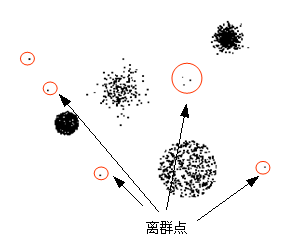
\includegraphics[width=0.85\linewidth]{figure/2-1}
	\caption{答辩系统跨职能流程图}
\end{figure}

在接下来的分析业务系统需求之后,用例图被整理出来,如图 2-2 所示。这再一次清晰地展示了系统的需求,便于进一步开发。用例图表示用户与系统的交互,表示用户与不同用例之间的关系。用例图可以识别系统的不同用户类型和不同的用例,并且通常还会附带其他类型的图表。

\begin{figure}
	\centering
	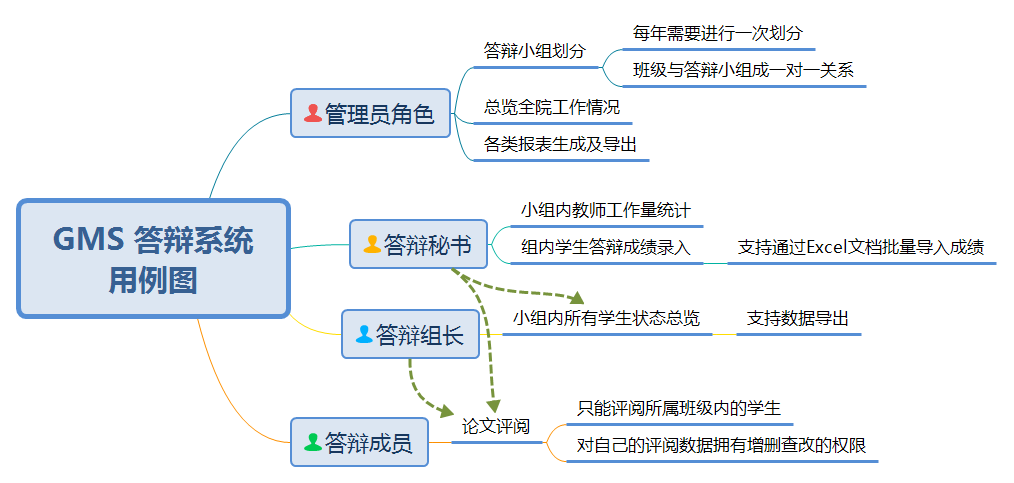
\includegraphics[width=0.85\linewidth]{figure/2-2}
	\caption{答辩系统用例图}
\end{figure}

虽然用例本身可能包含了关于每种可能性的大量细节,但用例图可以帮助提供更高级别的系统视图。用例图是软件系统开发的蓝图,它们提供了系统必须实际执行内容的图形表示。由于其简单性,用例图可以成为利益相关者的良好沟通工具。并且,用例图以更简化的方式将设计者的意图传达给利益相关者,并且拥有比类图更完整的细节。用例图的目的是提供系统的高级视图,提供系统的粗略功能和简单技术视图。


\subsection{数据库设计}

数据库设计是根据数据库模型组织数据的过程。设计者确定必须存储什么数据以及数据元素是如何相互关联的。有了这些信息,我们就可以开始将数据拟合到数据库模型中。数据库设计涉及分类数据和确定相互关系。这种关于数据的理论表示被称为本体论。本体论是数据库设计背后的理论。

在大多数情况下,设计数据库的人是在数据库设计领域具有专业知识的人,而不需要业务领域的专业知识,例如,教育经验,从医经验等。因此,数据库设计必须与在该领域具有专业知识的人员合作确定,以确定必须在系统内存储什么样的数据。这是因为具有必要领域知识的人员经常无法清楚地表达他们对数据库的系统要求是什么,因为他们不习惯于根据必须存储的离散数据元素进行思考。要存储的数据可以由需求规格确定。这个过程通常被认为是需求分析的一部分。

一旦数据库设计者确定要存储在数据库中的数据后,他们就必须确定数据间的依赖关系。例如,在姓名和地址列表中,假设多人可以拥有相同的地址,但一个人不能拥有多个地址的情况下,地址取决于姓名。当提供姓名时,地址可以唯一确定,然而,反过来并不成立 —— 当给定一个地址时,名称不能唯一确定,因为多个人可以居住在一个地址。由于地址是由名称决定的,所以地址被视为取决于名称。

大多数数据库设计文件采用 
E-R图\footnote{实体 - 关系模型(简称ER模型)描述了特定知识领域中相关的感兴趣事物。基本的ER模型由实体类型(对感兴趣的事物进行分类)组成,并指定可能存在于这些实体类型的实例之间的关系。}
或更直观的矢量图片表示。但是这些文件均是二进制文件,在基于 
Git\footnote{Git 是一个版本控制系统,用于跟踪计算机文件中的变化并协调多人之间的这些文件的工作。在后文还会详细介绍本项目基于 Git 的团队协作工作流。} 
的版本控制系统中,只能存储、共享,而不能进行高效的团队协作,所以在这次答辩系统的开发中,选用了以文本结构存储数据库设计(JavaScript 代码),让数据库设计文档在便于浏览阅读的同时,拥有了很好的团队协作编辑的能力。如代码 2-1 所示,是答辩系统数据库设计的主要部分。(意义不大的部分已省略)

值得一提的是,该项目使用了非关系型数据库 MongoDB,这与传统的关系型数据库有一些不同之处。这将在后文进行具体的介绍。

\clearpage

\begin{lstlisting}[title=代码 2-1:数据库设计]
const dbDesign = {
	// ...
	'inspectionGroup 答辩小组': [
		'_id',
		['index',           'int',      '从 1 开始的小组编号'],
		['year',            'int'],
		['leader_id',       'ID'],
		['secretary_id',    'ID'],
		['member_id',       'ID array'],
		['class_id',        'ID']
	],
	user: [
		'_id',
		['createdAt',   'Date'],
		['username',    'str',    '学号/工号'],
		['name',        'str',    '姓名'],
		['kind',        'int',    '人员类型'],
		['spr_id',      'ID',     '系主任或学生所属的专业'],
		['spr_name',    'str'],
		['profile',     'Object', '个人信息', [
			// ...
		],
		['services',    'meteor 存储的额外信息'],
		
		'---- 学生属性 ----',
		['stu_status',  'int', '状态'],
		['stu_year',    'int', '毕业年级'],
		['class_id',    'ID',  '所属班级'],
		['class_name',  'str'],
		'---- 教师属性 ----',
		['is_dean',             'bool', '系主任身份'],
		['tea_edit_time',       'Date', '额外允许教师编辑题目的期限'],
		['tea_level',           'str',  '职称'],
		['inspection_group_id', 'ID',   '所属答辩小组'],
		['inspection_role',     'int',  '在答辩小组中扮演的角色', '0非成员 1组长 2秘书 3成员'],
	]
};
\end{lstlisting}

